% igs2ejournalguide.tex
% v4.00 3-sept-2015

\NeedsTeXFormat{LaTeX2e}

% check that the math fits the two-column format:
 \documentclass[twocolumn,letterpaper]{igs}

% but use this version when submitting your article:
  %\documentclass[review,oneside]{igs}


  \usepackage{igsnatbib}
\usepackage{lmodern}
\usepackage{amsmath,amssymb,amsthm}
\usepackage{wrapfig}
\usepackage{enumitem}
\usepackage{multirow}
\usepackage{tabularx}
\usepackage{booktabs}
\usepackage{lscape}
\usepackage{color}
\usepackage{graphicx}
\usepackage{subcaption}





\begin{document}

\title[Optimizing snow survey design for winter balance]{Optimizing snow survey design for estimating winter balance of alpine glaciers}

\author[Pulwicki and Flowers]{Alexandra PULWICKI,$^1$
  Gwenn E. FLOWERS,$^1$}

\affiliation{%
$^1$ Department of Earth Sciences, Faculty of Science, Simon Fraser University, Burnaby, BC, Canada\\
  Correspondence: Alexandra Pulwicki 
  $<$apulwick@sfu.ca$>$}

%%%%%%%%%%%%%%%%%%%%%%%%%%%%%%%%%
%	ABSTRACT
%%%%%%%%%%%%%%%%%%%%%%%%%%%%%%%%%

%\abstract{Efficient collection of snow depth and density data is critical to a successful snow measurement campaign and to accurately estimate glacier winter balance. Since snow accumulation is spatially variable, snow properties must be measured over an extensive area within a short period of time. Extensive, high resolution and accurate snow accumulation measurements on glaciers are almost impossible to achieve so surveys need to optimize the extent and spacing of snow measurements to obtain reliable estimates of winter balance. To address this need, we estimate winter balance and root mean squared error (RMSE) using synthetic and real data from subsets of extensive surveys on three glaciers in the St. Elias Mountains, Yukon. We generate six different sampling designs, which encompass possible snow sampling patterns and various numbers of measurement locations. We then use linear regression with topographic parameters to interpolate measurements. Analysis of both synthetic and real data indicates that an `hourglass' shaped sampling design results in the most efficient and accurate estimate of winter balance, while the midline pattern results in poor estimates of WB for all glaciers. RMSE decreases with increased sample size, with no further reduction after about 30 measurement locations. When noise is added to synthetic data, 

%Winter balance estimates are 


%variable but not systematically affected by the measurement spacing. This study highlights the ability for future winter balance and snow survey studies to optimize snow data collection within a glacierized basin.

%\vspace{0.3cm} Keywords: {\normalfont glacier; alpine; snow survey design; optimize; St. Elias Mountains; snow probing}}

\maketitle

%%%%%%%%%%%%%%%%%%%%%%%%%%%%%%%%%
%	INTRODUCTION
%%%%%%%%%%%%%%%%%%%%%%%%%%%%%%%%%
\section{Introduction}

\begin{figure*}
	\centering
	\includegraphics[width =\textwidth]{PaperII-StudySite.pdf}\\
	\caption{Study area location and sampling design for Glaciers 4, 2 and 13. (Left) Study region in the Donjek Range of the St. Elias Mountains of Yukon, Canada (inset). Imagery from Landsat8 (29 August 2013, data available from the U.S. Geological Survey). (Right) Details of the snow-survey sampling design, with centreline and transverse transects (blue dots), hourglass and circle designs (orange dots) and locations of snow density measurements (green squares). Arrows indicate ice-flow directions. Approximate location of ELA on each glacier is shown as a black dashed line. Contour lines in increments of 50\,m are shown in grey.}
	\label{fig:Sampling}
\end{figure*} 

Estimates of basin-wide seasonal snow accumulation are critical for monitoring glacier mass balance and for predicting the availability and timing of surface runoff, especially in mountainous regions. The net accumulation and ablation of snow on a glacier over a winter season is known as the winter surface mass balance, or ``winter balance'' (WB) and is typically reported in meters of water equivalent (m\,w.e.) \citep{Cogley2011}. Winter balance accounts for half of the seasonally resolved mass balance, initializes ablation conditions and affects energy and mass exchange between the land and atmosphere \citep[e.g.][]{Hock2005, Reveillet2016}. 

Snow distribution is spatially variable so properties, such as snow depth, must be measured over an extensive area \citep[e.g.][]{Kinar2015}. In addition, the period of peak accumulation is short so snow measurement must be completed quickly and efficiently. As a result, representative measurements of snow depth are nearly impossible to obtain. Snow surveys must therefore be optimized in the extent and spacing of snow measurement locations, especially when labour-intensive methods like snow probing are used. 

Optimal sampling schemes for snow probing are central to accurately estimating snow distribution and mass balance from \textit{in situ} measurements. Measuring snow depth and travelling between measurement locations is both time consuming and can disturb the snow so care must be taken to choose a sampling scheme that avoids bias, allows for the greatest variability to be measured and minimizes distance travelled \citep{Shea2010}. There are a number of different designs that have been employed to obtain point measurements, including pure random \citep[e.g.][]{Elder1991}, linear random \cite[e.g.][]{Shea2010}, nested \citep[e.g.][]{Schweizer2008}, gridded random \citep[e.g.][]{Bellaire2008, Elder2009, Bellaire2011} and gridded \citep[e.g.][]{Molotch2005a, Kronholm2007, Lopez2011}. Sampling designs that incorporate randomness are favourable because they limit sampling bias by varying sample spacing and direction. However, they are less efficient than sampling designs that incorporate grids. Grid-style sampling designs minimize travel distance but measurements are biased by regularly spaced intervals and linear orientations, which could result in an under representation of the snow variability \citep{Kronholm2007}.

Snow surveys on glaciers are conducted to estimate winter balance and multi-year sampling programs are often established to monitor changes in winter balance with time. Optimization of sampling design is rarely investigated because the locations of snow depth measurements are often dictated by field resources. An optimized sampling design requires (1) a sampling pattern that captures spatial variability and minimizes travel distance and (2) knowledge of the minimum number of measurement locations needed to accurately estimate WB. There are few studies that investigate the number of measurement locations needed to effectively sample WB distribution \citep[c.f.][]{Fountain1999,Walmsley2015}. The sampling pattern used for most winter balance programs does not included randomness and measurements are typically collected along the glacier midline \citep[e.g.][]{Kaser2003} to capture changes in snow depth due to orographic effects \citep[e.g.][]{Grunewald2014}. However, midline transects are known to underestimate winter balance so transverse transects are often added to improve the reliability of the sampling scheme \citep[e.g.][]{Walmsley2015}. An hourglass with inscribed circle (personal communication from C. Parr, 2016) is an alternative sampling design that is attractive because it is able to capture changes in WB with elevation but is not biased along the midline and is easy to travel. To our knowledge, no study has yet compared the ability of these sampling designs to capture spatial variability in WB.  

The goal of our work is to provide insight into optimization of WB sampling design by investigating various sampling patterns and number of measurement locations. We use both synthetic- and real data to examine the effect of sampling design on estimates of glacier-wide WB for three alpine glaciers. 


%%%%%%%%%%%%%%%%%%%%%%%%%%%%%%%%%
%	STUDY SITE
%%%%%%%%%%%%%%%%%%%%%%%%%%%%%%%%%


\section{Study site}

We investigate sampling design for winter balance surveys on three unnamed glaciers in the Donjek Range of the St. Elias Mountains, Yukon, Canada. The Donjek Range is located on the continental side of the St. Elias Mountains, which rise sharply from the Pacific Ocean and create a strong climatic gradient. Monitoring of snow distribution and glacier mass balance in the St. Elias Mountains began in the 1950s and 60s with a series of research programs, including Project ``Snow Cornice''  and the Icefield Ranges Research Project \citep{Wood1948, Danby2003}. More recent studies have focused on glaciological studies of selected alpine glaciers \citep[e.g.][]{Clarke2014} as well as estimates of regional glacier mass balance and dynamics \citep[e.g.][]{Arendt2008, Burgess2013,Waechter2015}. 

Glacier 4, Glacier 2 and Glacier 13 (labelling adopted from \cite{Crompton2016}) are small alpine glaciers (3.8--12.6\,km$^2$) with simple geometries. Elevation of these glaciers ranges from 1900 to 3100\,m\,a.s.l. and ELAs are located at $\sim$2500\,m. The glaciers are generally oriented southeast-northwest in valleys with steep walls. We suspect that the glaciers are polythermal, based on a detailed study of Glacier 2 \citep{Wilson2013} and related theoretical modelling \citep{Wilson2013a}. A detailed analysis of estimating winter balance on these three glaciers is presented by \cite{Pulwicki2017}.

%%%%%%%%%%%%%%%%%%%%%%%%%%%%%%%%%
%	FIGURES & TABLES
%%%%%%%%%%%%%%%%%%%%%%%%%%%%%%%%%

\begin{figure*}
	\centering
	\includegraphics[width =0.9\textwidth]{SamplingDesignAll.pdf}\\
	\caption{Synthetic sampling designs on three study glacier. All synthetic observation measurement locations (small, black dots) and a subset including 15 measurement locations (open circles) is shown for each sampling pattern. The random sampling pattern shows a total of 200 sampling locations. Sampling designs are overlain on the prescribed winter balance (WB). } 
       \label{fig:SyntheticSampleDesign}
\end{figure*}

\begin{figure*}
	\centering
	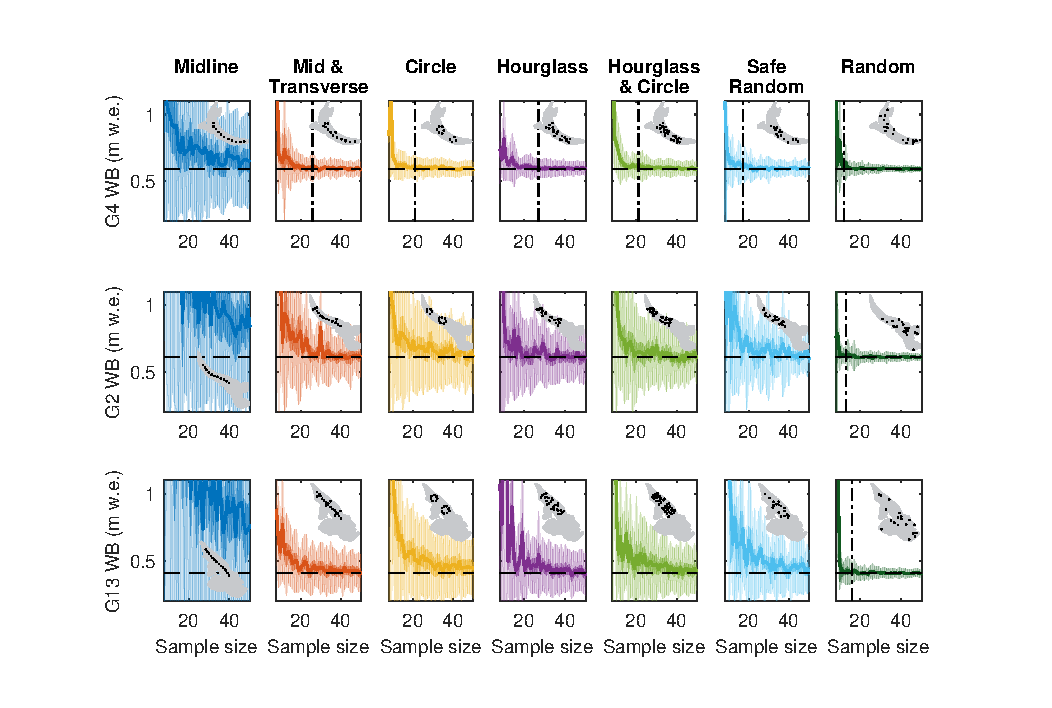
\includegraphics[width =\textwidth]{SyntheticObsWB.pdf}\\
	\caption{Glacier-wide winter balance (WB) estimated with various sampling designs for Glacier 4 (top row), Glacier 2 (middle row) and Glacier 13 (bottom row). Sampling patterns are shown in columns. Insets show an example of a sampling design corresponding to the panel. Mean WB from 100 runs of a linear regression of synthetic WB on topographic parameters for various patterns and sample sizes (solid coloured line) with second-order exponential fit (solid black line). Standard deviation in glacier-wide WB due to low noise (dark shading) and high noise (light shading). Glacier-wide WB of validation data (black dashed line). Sample size when fitted mean is within 0.05\,m\,w.e. of true mean (black dotted line) and when standard deviation due to high noise is less than 0.15\,m\,w.e. (black dotted-dashed line) are shown.}
	\label{fig:SyntheticObsWB}
\end{figure*}

\begin{table*}[]
\centering
\caption{Minimum travel distance (km) required to fulfil each sampling pattern. Distance for random design ($n=40$) is the sum of distances between closest measurement locations and a range is provided for an array of different random locations.}
\label{tab:DistanceTravelled}
\begin{tabular}{ccccccc}
\midrule
 & \textbf{Midline} & \textbf{\begin{tabular}[c]{@{}c@{}}Midline \&\\ Transect\end{tabular}} & \textbf{Circle} & \textbf{Hourglass} & \textbf{\begin{tabular}[c]{@{}c@{}}Hourglass\\ \& Circle\end{tabular}} & \textbf{Random} \\ \midrule
\textbf{Glacier 4} & 6.3 & 8.3 & 4.8 & 6.9 & 11.1 & 5.5--10.2 \\
\textbf{Glacier 2} & 4.3 & 8.6 & 5.7 & 8.4 & 12.5 & 6.6--11.8 \\
\textbf{Glacier 13} & 8.0 & 11.0 & 7.0 & 10.6 & 16.8 & 8.3--14.2
\end{tabular}
\end{table*}

\begin{figure*}
	\centering
	\includegraphics[width =\textwidth]{SynObsRMSEmap.pdf}\\
	\caption{Root-mean-squared-error (RMSE) between validation WB and WB estimated with various sample patterns ($n=40$) for 100 runs of high noise linear regression. Sampling patterns are shown in columns for Glacier 4 (top row), Glacier 2 (middle row) and Glacier 13 (bottom row). RMSE for the entire glacier is displayed. Synthetic sampling locations are shown (black dots).}
	\label{fig:SynObsRMSEmap}
\end{figure*}

\begin{figure*}
	\centering
	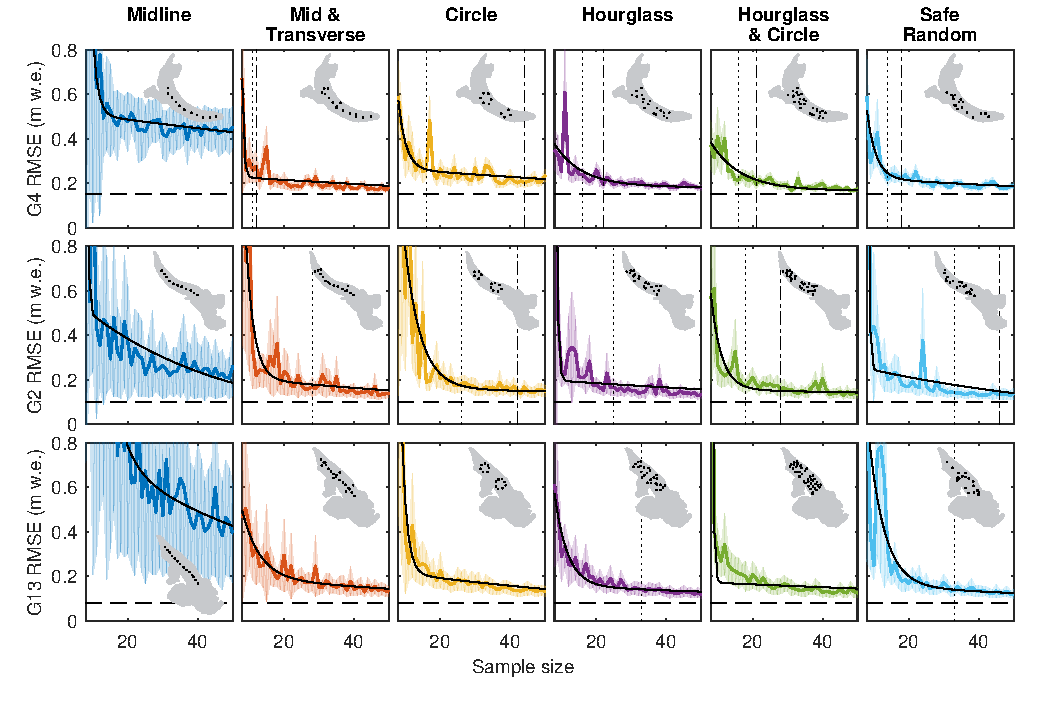
\includegraphics[width =\textwidth]{DataObsWB.pdf}\\
	\caption{Root-mean-squared-error (RMSE) between WB estimated with various sampling designs of real data and field values of WB at all measurement locations for Glacier 4 (top row), Glacier 2 (middle row) and Glacier 13 (bottom row). Sampling patterns are shown in columns. Insets show an example of a sampling design corresponding to the panel. Mean RMSE from 100 runs of a linear regression of real WB on topographic parameters for various patterns and sample sizes (solid coloured line) with second-order exponential fit (solid black line). Standard deviation in RMSE due to low noise (dark shading) and high noise (light shading). RMSE of estimated WB when all measurement locations are used in the linear regression (black dashed line). Sample size when fitted RMSE mean is within 0.05\,m\,w.e. of true RMSE mean (black dotted line) and when standard deviation due to high noise is less than 0.01\,m\,w.e. (black dotted-dashed line) are shown.}
	\label{fig:RealObsWB}
\end{figure*}

%%%%%%%%%%%%%%%%%%%%%%%%%%%%%%%%%
%	METHODS
%%%%%%%%%%%%%%%%%%%%%%%%%%%%%%%%%

\section{Methods}

We aim to determine the optimal sampling pattern and number of measurement locations needed to obtain accurate estimates of WB for small alpine glaciers. We estimate distributed WB using both synthetic- and real values of gridcell WB. Real data are subsets of all gridcell values of WB, which is derived from direct measurements of snow depth and density, chosen based on different sampling designs. A linear regression is used to interpolate gridcell values resulting in an estimated WB. Synthetic data are generated by sampling a synthetic distribution of WB, which is based on field measurements, using various sampling designs. Uncertainty in gridcell WB is incorporated by introducing noise into the synthetic distribution of WB. A linear regression of synthetic data on topographic parameters is then used to estimate WB. A set of estimated WB is generated by repeating this process with different levels of noise. We then directly compare the estimated WB and the synthetic distribution of WB.  Three study glaciers, with differing spatial patterns of WB, are used to determine the applicability of our conclusions between glaciers. 

Here we describe the process of collecting WB data in the field and interpolating/extrapolating to obtain the synthetic distribution of WB on the three study glaciers. Subsets of the real data are used to investigate the effect of various sampling designs on the error associated with estimating gridcell-scale values of WB. Then, we detail the methods used to obtain synthetic data and describe the various sampling patterns and number of measurement locations investigated in this study. A comparison of the synthetic distribution of WB and WB estimated using different sampling designs with synthetic data is presented. 

\subsection{Field data}

Point-scale values of WB are found by obtaining direct measurements of snow depth and density (Figure \ref{fig:Sampling}). Snow depth was measured using a 3.2\,m graduated aluminium avalanche probe. Measurement locations followed linear and curvilinear transects, which were similar between study glaciers, with a sample spacing of 10--60\,m.  Spacing was constrained by protocols for safe glacier travel. Each observer made 3--4 depth measurements within $\sim$1\,m at each transect measurement location. We restricted snow-depth sampling to the ablation area, where the clear distinction between snow and ice ensured that only snow from the current accumulation season was measured. In total, we collected more than 9000 snow-depth measurements throughout the study area. Snow density was measured using a wedge cutter in three snow pits that spanned a large portion of the elevation on each glacier. A mean density was then calculated for each glacier and this value was used to convert snow depth at all measurement locations to values of point-scale WB. Mean density was 348$\pm$13\,kg\,m$^{-3}$ on Glacier 4, 333$\pm$26\,kg\,m$^{-3}$ on Glacier 2 and 349$\pm$38\,kg\,m$^{-3}$ on Glacier 13. All point-scale values of WB located within a common DEM gridcell ($40\times40$\,m) were averaged to obtain values of gridcell WB. 

\subsection{Real data}

Sampling designs are derived from all measurement locations for each study glacier (Figure \ref{fig:Sampling}). We investigate numerous sampling designs that are unique combinations of six different sampling patterns and the number of measurement locations. Midline and midline \& transverse transects are the most common survey designs used in WB studies \citep[e.g.][]{Kaser2002, Machguth2006}. The midline survey aims to capture changes in WB with elevation and transverse transects provide observation of lateral variations in WB. Hourglass and inscribed circle allow for sampling in multiple directions and are easy to travel (personal communication from C. Parr, 2016). We use hourglass and circle patterns separately and combined. Finally, a random pattern of measurement locations is obtained by selecting random gridcells from the full data set. For all sampling patterns we estimate WB using $n$ measurement locations, where $n$ ranges from a minimum of eight (constrained by using all seven topographic parameters for interpolation) to a maximum determined by the number of gridcells within a sampling pattern (ranges between 57--228 gridcells). The measurement locations are evenly distributed within the sampling pattern. 

A linear regression is then used to interpolate the real values of WB for each glacier. Real data is regressed on elevation, slope, aspect, distance from glacier centreline, ``northness'', curvature and a wind redistribution parameter. The linear regression calculates regression coefficients that minimize the sum of squares of the vertical deviations of each datum from the regression line \citep{Davis1986}. The resulting regression coefficients are then applied to the topographic parameters associated with each gridcell to obtain an estimate of distributed WB. Results are presented as a RMSE value, which is calculated by taking the square root of the mean difference between WB estimated using various sampling designs and real data at all measurement locations.


\subsection{Synthetic data}

We obtain synthetic data using various sampling designs from the synthetic distribution of WB to test which sampling design best estimates WB. Gridcell values of WB that fall within each sampling design are extracted from the synthetic distribution of WB distribution and then used to estimate a new WB distribution. The WB distribution derived from various sampling designs is directly compared to the synthetic distribution of WB distribution to estimate spatially resolved error. 

The synthetic distribution of WB is obtained by computing a linear regression of gridcell values of WB on topographic parameters for each glacier \citep{Pulwicki2017}. Topographic parameters are derived from a SPIRIT SPOT-5 DEM \citep{Korona2009} and include commonly applied topographic parameters \citep[e.g.][]{McGrath2015} such as elevation, slope, aspect, distance from glacier centreline, ``northness'', curvature and a wind redistribution parameter. A linear regression, along with cross-validation and model averaging, is used to obtain a set of regression coefficients for the standardized topographic parameters on each glacier \citep{Pulwicki2017}. Distributed WB is found by multiplying fitted regression coefficients by corresponding topographic parameters for each gridcell. The distributed WB calculated using all available WB data is hereafter referred to as the synthetic distribution of WB.

Synthetic data are obtained for all of the sampling designs presented above. Midline, midline \& transects, circle, hourglass, hourglass \& circle and random sampling patterns are used (Figure \ref{fig:SyntheticSampleDesign}) and values of $n$ from eight to the maximum number of observation with each sampling pattern are investigated. All sampling patterns are restricted to the ablation area, where terrain is accessible and direct measurements of snow depth are easy to obtain. The random pattern selects measurements locations within the area that encompasses the original sampling designs.

To simulate the process of measuring WB, we first obtain WB values from the synthetic distribution of WB distribution at selected measurement locations for each sampling pattern. Then, we add a low or high level of noise to the WB data. Low noise is defined by a normal distribution that is centred at zero and has a standard deviation equal to the mean standard deviation of WB data from a series of high-density gridcell-scale surveys on each glacier \citep{Pulwicki2017}. High noise is defined in the same way as low noise but the standard deviation of the normal distribution is three times larger, which is approximately equal to the standard deviation of the WB probability distribution that accounts for uncertainty due in grid-scale WB, density assignment, and interpolation for the three study glaciers \citep{Pulwicki2017}. For each gridcell value of WB, a random number from the high or low noise distribution is added to obtain a synthetic observation of WB.

As above, a linear regression is calculated between synthetic data and topographic parameters and an estimated WB is then calculated. The process of adding random noise to gridcell-scale values of WB to obtain synthetic observations and fitting a regression to then estimate distributed WB is repeated 100 times to create a population of possible WB estimates. Each repetition uses a different set of random noise resulting in a range of WB values from which a mean WB and RMSE is then calculated. RMSE is found by taking the square root of the mean difference between all gridcells in the synthetic distribution of WB distribution and the WB distribution derived with the sampling design.
 
 \subsection{Performance metrics}
 
To quantify the performance of each sampling pattern, we use two performance metrics. The first metric is `convergence', which is defined as the number of measurement locations ($n$) needed to obtain a mean WB within 5\% of the synthetic glacier-wide WB or the RMSE for WB estimated using all real data points. The relation between WB or RMSE and $n$ is smoothed (...describe it here). Convergence is a metric that describes the minimum number of measurement locations required to have an accurate estimate of WB. The second metric is `variability' (or `sensitivity'?), which is defined as the number of measurement locations required to have the standard deviation of WB or RMSE due to high noise within 5\% of the synthetic glacier-wide WB or the RMSE for WB estimated using all real data points. Again, the curve is smoothed. Variability is a metric of how sensitive the WB estimate is to uncertainty in grid-scale variability and interpolation. The total distance required to obtain measurements along a sampling pattern from a central location is also presented. An efficient sampling design would have lower $n$ values for convergence and variability metrics as well as a short travel distance. 

%%%%%%%%%%%%%%%%%%%%%%%%%%%%%%%%%%%%%%%%%%%
%%  RESULTS
%%%%%%%%%%%%%%%%%%%%%%%%%%%%%%%%%%%%%%%%%%%
\section{Results }

\subsection{Synthetic data}

Based on synthetic data, the most effective sampling patterns are midline \& transect and hourglass for all three study glaciers. Midline \& transect and hourglass quickly converge to the validation value of WB, have comparatively low standard deviations due to noise and involve the shortest travelling distances (Figure \ref{fig:SyntheticObsWB} and Table \ref{tab:DistanceTravelled}). To estimate a mean WB within 5\% of the synthetic distribution of WB, $\sim$5 fewer measurements are needed for the midline \& transect design as compared to the hourglass design while travelling distance is slightly shorter for the hourglass design. The variability in WB estimates due to high noise becomes small ($<0.15$\,m\,w.e.) when $n>25$.

The remaining sampling patterns are less effective for estimating WB. Hourglass \& circle and random sampling patterns also require small sample sizes but the standard deviations due to noise are larger and travelling distance is substantially greater. Further, the mean WB does not converge to the synthetic distribution of WB for $n<50$ on Glaciers 2 and 13. Notably, hourglass \& circle is not a substantial improvement on the hourglass sampling pattern given the considerable increase in travel distance required to sample the along the hourglass \& circle. The circle pattern is not a reliable method of sampling because the standard deviation due to noise is comparatively high and the mean WB does not conver to the synthetic distribution of WB on Glaciers 2 and 13. By far the worst sampling pattern is the midline. WB values are highly sensitive to noise and even with a large number of measurement locations the validation values of WB are not achieved. 

Although the convergence patterns are similar between glaciers, the standard deviation due to noise and the number of measurement locations needed to accurately estimate WB are smallest for Glacier 4 and greatest for Glacier 13 for all sampling patterns. With all sampling patterns, WB is significantly overestimated at low $n$. If using midline \& transect or hourglass sampling patterns, a sampling size of $\sim$20 is sufficient to estimate glacier-wide WB with no marked improvement in accuracy or precision at larger sample sizes. 
Error in estimated WB is generally greatest in the accumulation area, especially for Glaciers 2 and 13 (Figure \ref{fig:SynObsRMSEmap}). When midline pattern is used, the errors are exceptionally high in areas that do not fall along the midline.

\subsection{Real data}

The RMSE rapidly decreases with an increased sample size for all sampling patterns on all three glaciers (Figure\ref{fig:RealObsWB}).  The sampling patterns trends are similar to those of the synthetic data. Midline \& transverse, hourglass, hourglass \& circle and random all perform well. However, the higher travelling distance of hourglass \& circle and random make these patterns less efficient. Circle pattern appears to perform quite well although RMSE values are slightly higher. Again, the worst pattern is the midline, which results in exceptionally high values of RMSE. 

An appropriate sample size is more difficult to determine based on sampling designs from real data. For all glaciers, $n>30$ does not result in a marked decrease in RMSE. However, none of the sampling patterns result in the RMSE reaching that of the full data for $n<50$. 

%%%%%%%%%%%%%%%%%%%%%%%%%%%%%%%%%%%%%%%%%%%
%% DISCUSSION
%%%%%%%%%%%%%%%%%%%%%%%%%%%%%%%%%%%%%%%%%%%
\section{Discussion}

The optimal sampling design for our study region is the hourglass pattern with a sample size of $\sim30$. Based on both synthetic and real data, this design results in low error, is least sensitive to noise and involves relatively small travelling distance. The more broadly applied midline \& transverse pattern also produces reliable WB estimates but is slightly less efficient for travelling. A sample size greater than 30 does not significantly improve the accuracy of WB estimated and does not decrease error. This surprisingly low number of measurement locations indicates that high-resolution sampling is not required to accurately estimate WB. Instead, taking measurements throughout the study basin should be prioritized when choosing a sampling design. If the goal is to estimate WB then field resources should be more strongly allocated to distributing measurement locations to capture basin-scale spatial trends in WB. Error is greatest in areas far from sampling locations and in areas with extreme values of topographic parameters. 

The most effective sampling designs capture the dominant WB-elevation trend but also have measurement locations in gridcells that span the range of other topographic parameters. Despite the fact that the synthetic distribution of WB on Glaciers 2 and 13 is largely controlled by elevation, measurements locations that are not along the midline are needed to constrain the regression. When the midline pattern is used, the topographic parameters excluding elevation fall within a narrow range so the regression becomes sensitive to noise. Further, the accuracy of estimated WB does not improve at large $n$ along a midline pattern because the sampling locations do not capture relationships between WB and the remaining topographic parameters. However, if there are a large portion of measurement locations far from the midline then the elevation trend may be less strong resulting in larger errors. Random and hourglass \& circle patterns may have larger errors on Glaciers 2 and 13 as a result of the higher proportion of measurement locations far from the midline. 

On Glacier 4, the standard deviation of WB due to noise and the number of measurement locations needed to estimate WB is smaller than Glaciers 2 and 13. This trend is likely a result of the small influence of topographic parameters in the distribution of synthetic distribution of WB. The synthetic distribution of WB is derived from a linear regression between field measurements of WB and topographic parameters that explains little of the observed variance (R$^2=$0.07). As a result, glacier-wide WB is approximately equal to the mean of WB field measurements. This mostly uniform distribution of snow can therefore be described with few measurement locations, regardless of where the measurements are obtained. 

Further work into the optimization of snow survey sampling design is needed. The most obvious limitation of our study is the restriction of sampling design to accessible locations in the ablation area. Lack of measurements in the accumulation area is a sub-optimal sampling design. However, direct measurements of snow depth in the accumulation area are extremely costly because a large amount of time is needed to dig a snow pit, especially in regions with high accumulation. Given the importance of spatially distributed measurements though, there is likely an optimal balance between costly measurements in the accumulation area and less costly measurements in the ablation area. Use of more efficient snow-depth measurement methods, such a ground-penetrating radar (GPR) and lidar, in the accumulation area can also be investigated. Additional extensions to our work include an invetigation of the size and placement of hourglass patterns and to optimize measurement locations based on factors such as topographic parameters. 

low n over estiamtes


%%%%%%%%%%%%%%%%%%%%%%%%%%%%%%%%%%
% CONCLUSION
%%%%%%%%%%%%%%%%%%%%%%%%%%%%%%%%%%
\section{Conclusion}


\section{Acknowledgements}

We thank the Kluane First Nation (KFN), Parks Canada and the Yukon Territorial Government for granting us permission to work in KFN Traditional Territory and Kluane National Park and Reserve. We are grateful for financial support provided by the Natural Sciences and Engineering Research Council of  Canada, Simon Fraser University and the Northern Scientific Training Program. We kindly acknowledge Kluane Lake Research Station, Sian Williams, Lance Goodwin and Trans North pilot Dion Parker for facilitating field logistics. We are grateful to Alison Criscitiello and Coline Ariagno for all aspects of field assistance and Sarah Furney for assistance with data entry. Thank you to Etienne Berthier for providing us with the SPIRIT SPOT-5 DEM and for assistance in DEM correction. We are grateful to Derek Bingham and Michael Grosskopf for assistance with statistics. 

% all provided thoughtful and constructive comments on drafts of the manuscript.


%----------------------------------------------------------------------------------------
%	REFERENCE LIST
%----------------------------------------------------------------------------------------
%
%\bibliography{MastersLit}
\bibliography{/home/glaciology1/Documents/MastersDocuments/MastersLit}
%\bibliography{/Users/Alexandra/Documents/SFU/MastersDocuments/MastersLit}
\bibliographystyle{igs}

%----------------------------------------------------------------------------------------

\end{document}
